\documentclass{article}
%przykladowe pakiety
\usepackage[utf8]{inputenc}
\usepackage{polski}
\usepackage{graphicx}
\usepackage{amsmath} % w zasadzie tez mozna wywalic 
\usepackage{booktabs}
\usepackage{listings}
\usepackage{color}


% przykladowe kolorowanie kodu w listingu
\lstset{language=C++,backgroundcolor=\color[rgb]{0.99,0.99,0.99},captionpos=b,tabsize=3,numbers=left,numberstyle=\tiny,numbersep=5pt,basicstyle=\footnotesize,keywordstyle=\color[rgb]{0,0,1},commentstyle=\color{Darkgreen},stringstyle=\color{red},numbers=left,xleftmargin=2em,framexleftmargin=1.8em,}



\begin{document}

%strona tytulowa - osobny plik
\begin{titlepage}
    \newcommand{\HRule}{\rule{\linewidth}{0.5mm}}
    \center
    
\includegraphics[scale=0.4]{logo.jpg}\\[1cm] 
    \HRule \\[0.8cm]
    { \Large \bfseries 	 Projektowanie efektywnych algorytmów }\\[0.4cm]
    \HRule \\[1.5cm]
    { \Large \bfseries Projekt \textit{2}}\\[0.4cm]
    \textbf{ }
    \vspace{10mm} 
    
    \begin{minipage}{0.4\textwidth}
    \begin{flushleft} \large
    \end{flushleft}
    \end{minipage}
    \begin{minipage}{0.5\textwidth}
    \begin{flushright} \large
    \vfill
    \vspace{10mm} % mm vertical space
    \par Wydział Elektroniki
    \par Kierunek: Informatyka
    \vfill
    \par Paweł \textsc{Szynal 226026} \\
    \vspace{10mm} % mm vertical space
   \vspace{10mm} % mm vertical space
   \par Prowadzący:\\ mgr inż. Antoni Sterna
    \end{flushright}
    \end{minipage}\\[3cm]
     {\large Wrocław 2020 r.}\\[2cm]
\end{titlepage}
   
\newpage
    
\tableofcontents
\newpage

\section{Wstęp}

Zadaniem projektowym była implementacja dla problemu komiwojażera algorytmu Symulowanego Wyżarzania (ang. Simulated Annealing) sprawdzenie efektywności algorytmu, a także wyznaczenie błędu względnego (porównując z najlepszym znanym rozwiązaniem). 


\section{Symulowane wyżarzanie}

Algorytm Symulowanego Wyżarzania jest szczególnym przypadkiem algorytmu genetycznego. Nawiązuje do zjawiska fizycznego - zastygania cieczy tworzącej uporządkowaną, krystaliczną strukturę. W wysokiej temperaturze cząsteczki cieczy poruszają się swobodnie, ale wraz ze spadkiem temperatury możliwości ruchowe oraz prędkość poruszania się cząsteczek spada. Operacja powolnego schładzania ma na celu doprowadzenie metalu do równowagi termodynamicznej w stosunku do stanu wyjściowego oraz osiągnięcie pożądanych cech. Cały proces jest sterowany przez parametr zwany temperaturą.

Dla każdej iteracji wyznaczana jest nowa temperatura, która jest wyliczana wzorem T=T*s, gdzie s to sztywno zadana przez nas stała. Jest to sposób geometryczny wyznaczania temperatury.  Iteracje wykonują się dopóki wyliczona temperatura jest większa od sztywno zadanej w kodzie temperatury końcowej (w programie użyta wartość temperatury końcowej Tk = 0.01). Taka niska temperatura końcowa sprawia, że niemal niemożliwa jest zmiana rozwiązania na gorsze. Wielkość stałej s wpływa na szybkość schładzania jak i  na długość wykonywania algorytmu.


\section{Pomiary}

\subsection{Pomiary SW dla instancji z pierwszego projektu}
\begin{table}[h!]
\centering
\begin{tabular}{||c c c c||} 
\textbf{Rozmiar} & \textbf{Uzyskane średnie rozwiązanie} & \textbf{Czas {[}ms{]}} & \textbf{Błąd względny {[}\%{]}} \\
tsp\_10          & 215                                   & 190                    & 1\%                             \\
tsp\_15          & 307                                   & 242                    & 5,49\%                          \\
tsp\_17          & 41                                    & 261                    & 5\%                            
\end{tabular}
\caption{Pomiary SW dla instancji z pierwszego projektu}
\label{table:1}

\end{table}
\newpage


\begin{figure}[ht]

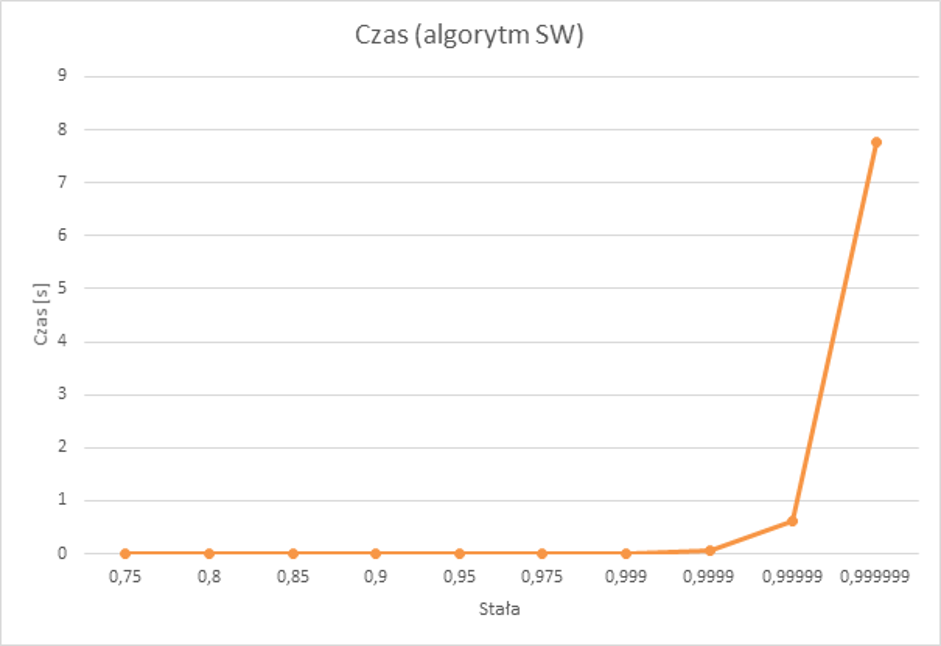
\includegraphics[width=1\textwidth]{./SW.png}
\caption{Pomiary dla instancji ftv47}

\end{figure}

\begin{figure}[ht]

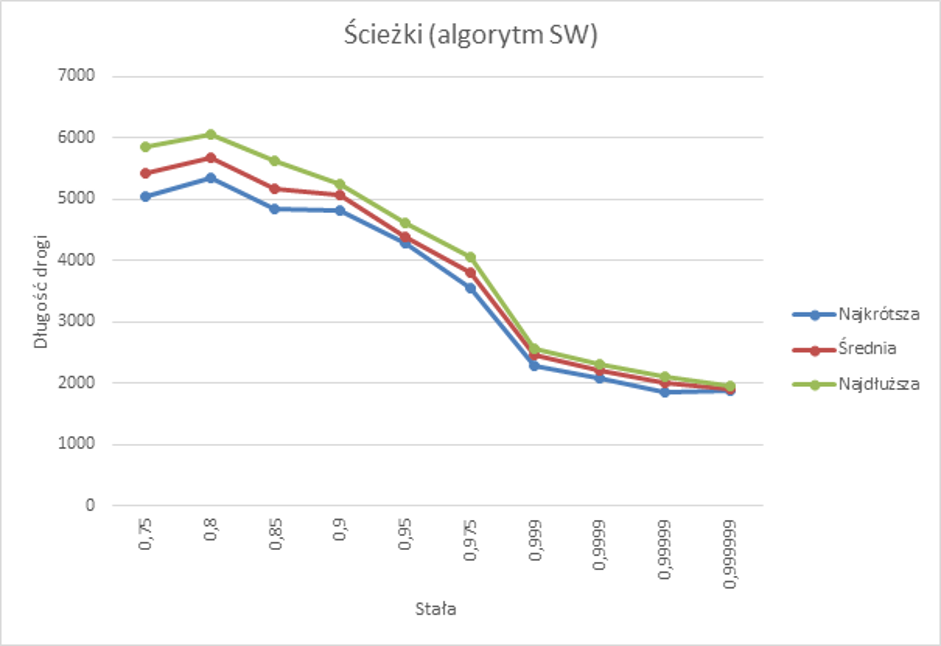
\includegraphics[width=1\textwidth]{./SW2.png}
\caption{Pomiary dla instancji ftv47}

\end{figure}

\section{Wnioski}

Algorytm nie gwarantuje uzyskania najlepszej drogi. Jego Ich wadą jest mała losowość - mimo tych samych parametrów jest możliwe uzyskanie różnych wyników - zależy to między innymi od początkowej permutacji drogi. Dużym plusem tych algorytmów metaheurystycznych jest możliwe uzyskanie przybliżonej odpowiedzi na zadany problem w akceptowalnym czasie. Porównując je do rozwiązań problemu komiwojażera z projektu pierwszego tego przedmiotu można łatwo zauważyć, że błąd względny wynosi maksymalnie 10\% (przy instancji 17 miast, czas wykonywania algorytmów poniżej 1s).
Czasu wykonania algorytmu jest proporcjonalny do ilości miast. Jest to związane choćby z najprostszą operacją obliczania długości drogi, która podczas jednej iteracji jest wykonywana wielokrotnie.
Algorytm po znalezieniu lokalnego minimum (które może być minimum globalnym), stara się szukać innej, bardziej optymalnej drogi. Mechanizm ten ma za zadanie zapobiec utknięciu w lokalnym minimum.
Zaletą algorytmu symulowanego wyżarzania jest mała złożoność pamięciowa.

\end{document}

